\documentclass[11pt]{beamer}
\usepackage[ngerman]{babel}
\usepackage{float}
\usepackage{graphicx}
\usepackage{caption}
\usepackage{hyperref}
\usepackage{cleveref}
\usepackage{fancyvrb}
\usepackage[%
  backend=bibtex,
  style=numeric]{biblatex}
\captionsetup{justification=centering}
\addbibresource{bib.bib}
\author{Maximilian Heim\inst{1}}
\beamertemplatenavigationsymbolsempty
\beamerdefaultoverlayspecification{<+->}
\AtBeginSubsection[]
{
    \begin{frame}
        \frametitle{Table of Contents}
        \tableofcontents[currentsection,currentsubsection]
    \end{frame}
}
\usetheme{Madrid}
\usecolortheme{whale}
\institute[HS-AS]
{
  \inst{1}
  Hochschule Albstadt-Sigmaringen
}
\crefname{section}{Kapitel}{Kapitel}
\crefname{figure}{Abbildung}{Abbildung}
\title{Identitäts- und Berechtigungsmanagement}
\date[IT-GRC 2024]{IT-GRC Seminar, Juni 2024}
\begin{document}
\frame{\titlepage}
\begin{frame}
  \frametitle{Gliederung}
  \tableofcontents
\end{frame}
\section{Identitätsmanagement- und Berechtigungsmanagement}
\subsection{Identitätsmanagement}
\begin{frame}
  \frametitle{Identität im Kontext des Identitätsmanagements}
  \begin{itemize}
    \item Unterschiedliche Definitionen
    \item Identitätsmanagement: Digitale Identität
    \item Digitale Identität: Bezeichner, Zugangsdaten und Attribute\footfullcite{bertino2010identity}
    \item Wichtig: Digitale Identitäten sind nicht nur Personen
  \end{itemize}
\end{frame}

\begin{frame}
  \frametitle{Digitale Identität}
  \begin{figure}[H]
    \centering
    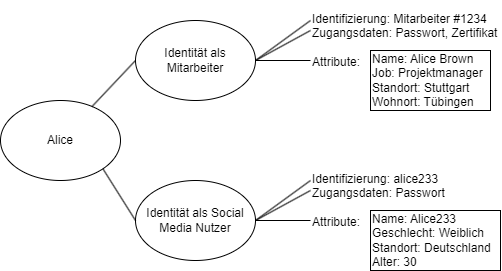
\includegraphics[width=0.7\textwidth]{assets/identity.png}
    \caption{Digitale Identität - Basierend auf Grafik 2.1 aus \glqq{}Identity Management Concepts, Technologies, and Systems\grqq{} von Elisa Bertino und Kenji Takahashi}
  \end{figure}
\end{frame}
\begin{frame}
  \frametitle{Identitätsmanagement}
  \begin{itemize}
    \item Management von digitalen Identitäten
    \item Aufgabenbereiche: Umfangreich
    \item Grundlegender Prozess: Identitätslebenszyklus
  \end{itemize}
\end{frame}

\begin{frame}
  \frametitle{Identitätslebenszyklus}
  \begin{figure}[H]
    \centering
    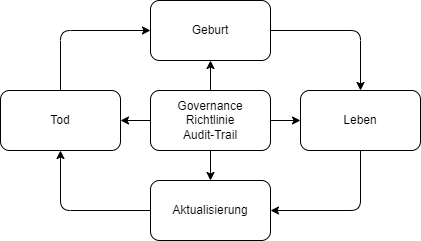
\includegraphics[width=0.6\textwidth]{assets/idlc.png}
    \caption{Identitätslebenszyklus - Basierend auf Grafik 2.3 aus \glqq{}Identity Management Concepts, Technologies, and Systems\grqq{} von Elisa Bertino und Kenji Takahashi}\label{fig:idlc}
  \end{figure}
\end{frame}

\begin{frame}<4->
  \frametitle{Identitätslebenszyklus}
  \begin{columns}
    \begin{column}{0.7\textwidth}
      \begin{figure}[H]
        \centering
        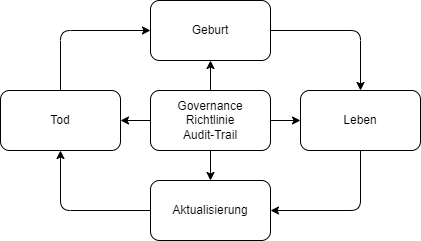
\includegraphics[width=0.6\textwidth]{assets/idlc.png}
        \caption{Identitätslebenszyklus - Basierend auf Grafik 2.3 aus \glqq{}Identity Management Concepts, Technologies, and Systems\grqq{} von Elisa Bertino und Kenji Takahashi}\label{fig:idlc}
      \end{figure}
    \end{column}
    \begin{column}{0.3\textwidth}
      \begin{itemize}
        \item Geburt: Datensammlung und Validierung, Zugangsdaten
        \item Leben: Authentifizierung, Weitergabe
        \item Änderung: Änderungen, Zugangsdaten
        \item Tod: Kündigung, Löschung
        \item Governance: Richtlinien, Audit-Trail
      \end{itemize}

    \end{column}
  \end{columns}
\end{frame}

\subsection{Berechtigungsmanagement}
\begin{frame}
  \frametitle{Berechtigung}
  \begin{itemize}
    \item Kombination aus Ressource und Operation~\footfullcite{tsolkas2017}
    \item Beispiele:
          \begin{itemize}
            \item Wer darf Inhalte des \textbackslash{}\textbackslash{}ad.hochschule.de Verzeichnisses ändern?
            \item Wer darf in Azure DevOps Repositories löschen?
            \item Wer darf in AWS Zertifikate erstellen?
            \item Wer darf das Wohnheim in der Poststraße 22 betreten?
          \end{itemize}
  \end{itemize}
\end{frame}

\begin{frame}
  \frametitle{Berechtigungsmanagement}
  \begin{itemize}
    \item Management von Berechtigungen: Welche Nutzer oder IT-Systeme (digitale Identitäten) dürfen auf welche Ressourcen zugreifen?
    \item Aufgaben:
          \begin{itemize}
            \item Wie werden Berechtigungen unterteilt? (Berechtigungskonzept - RBAC, ABAC, Kombination)
            \item Wie werden Berechtigungen vergeben und entzogen, wie werden irreguläre Berechtigungen vergeben?
            \item Wie werden Berechtigungskontrollen technisch umgesetzt? (Authorisierung)
          \end{itemize}
  \end{itemize}
\end{frame}

\subsection{Identitäts- und Berechtigungsmanagement}
\begin{frame}
  \frametitle{Identitäts- und Berechtigungsmanagement-Systeme}
  \begin{figure}[H]
    \centering
    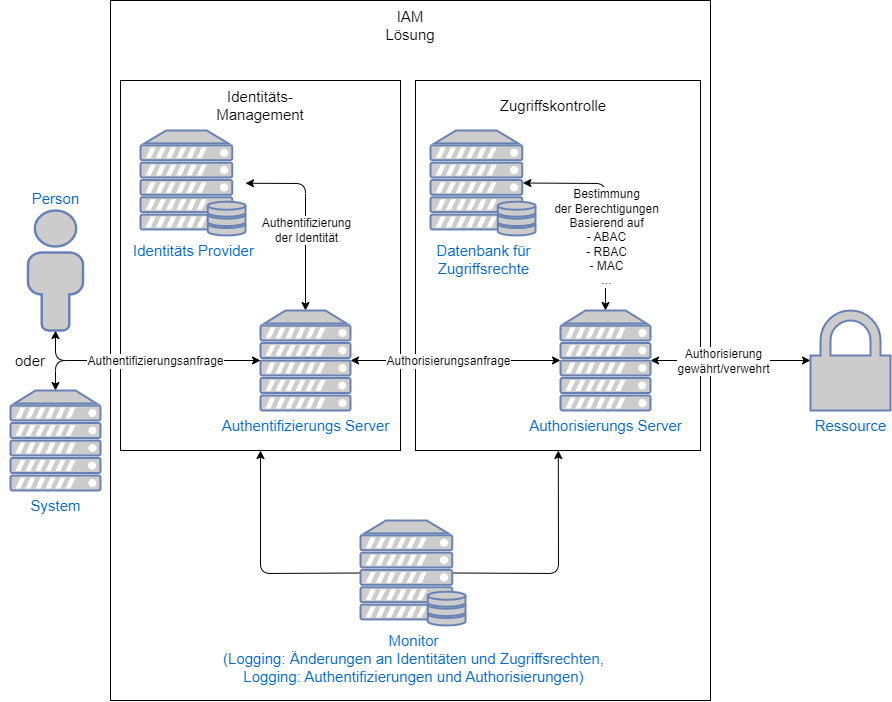
\includegraphics[width=0.7\textwidth]{assets/accessmanagement2.png}
    \caption{IAM System - Basierend auf Grafik 1 aus \glqq{}Identity and access management using distributed ledger technology: A survey\grqq{} von Fariba Ghaffari, Komal Gilani, Emmanuel Bertin und Noel Crespi}\label{figure:iam}
  \end{figure}
\end{frame}

\section{Betriebliches Identitäts- und Berechtigungsmanagement}

\subsection{Operative Aspekte}
\begin{frame}
  \frametitle{Operative Aspekte}
  \begin{itemize}
    \item CIO: Planung und Leitung der benötigten IT-Systeme
    \item CISO: Bewertung der Prozesse, Überwachung der Compliance mit Datenschutzstandards und Sicherheitsstandards, Awareness Trainings, interne Audits...
    \item IT-Betrieb: Implementierung und Wartung der involvierten Technik
    \item Personalabteilung: Identity-Lifecycle Management
    \item Helpdesk: Hilfe bei Authentifizierung und Authorisierung
  \end{itemize}
\end{frame}

\subsection{Technische Aspekte}
\begin{frame}
  \frametitle{Technische Aspekte}
  \begin{itemize}
    \item Produkte von Konzernen wie Microsoft, SAP, IBM, Okta \ldots
          \begin{itemize}
            \item Cloud (IDaaS - Identity as a Service) vs. On Premise
            \item Prozesse: Automatisiertes Lifecycle Management, Risikoanalyse, Audit
            \item Technologie: Multi Faktor Authentifizierung, Single Sign On
            \item Integration: Active Directory, Microsoft Office, AWS, HR Anwendungen
            \item \ldots
          \end{itemize}
  \end{itemize}
\end{frame}

\begin{frame}
  \frametitle{Technische Aspekte}
  \begin{figure}[H]
    \centering
    \includegraphics<1>[width=0.9\textwidth]{assets/Entra.png}
    \includegraphics<2>[width=0.9\textwidth]{assets/Verify.png}
    \includegraphics<3>[width=0.75\textwidth]{assets/Workforce.png}
    \caption{\only<1>{Microsoft Entra ID - von \url{https://www.microsoft.com/de-de/security/business/microsoft-entra}}\only<2>{IBM Security Verify - von \url{https://www.ibm.com/de-de/products/verify-saas}}\only<3>{Okta Workforce Identity Cloud - von \url{https://thectoclub.com/tools/best-identity-and-access-management-solutions/}}}
  \end{figure}
\end{frame}

\subsection{Compliance}
\begin{frame}
  \frametitle{Rechtlich}
  \begin{itemize}
    \item EuroSOX: Berechtigungskontrolle, Funktionstrennung
    \item KonTraG: Risikomanagementsystem
    \item GoBD: Berechtigungskontrollen, Nachvollziehbarkeit von Änderungen
    \item EU-DSGVO und BDSG: Speicherung, Verarbeitung und Weitergabe von personenbezogenen Daten
    \item ...
  \end{itemize}
\end{frame}

\begin{frame}
  \frametitle{Standards}
  \begin{itemize}
    \item ISO 27001: Annex A.9 definiert Zugangssteuerung
    \item IT-Grundschutz: BSI-Standard 200-1, ORP.4
    \item NIST 800-53A: Kapitel Access Control Family (AC) und Identification and Authentication Family (IA)
    \item ...
  \end{itemize}
\end{frame}

\begin{frame}
  \frametitle{Fragen}
  \begin{itemize}
    \item Vielen dank für eure Aufmerksamkeit!
    \item Fragen?
  \end{itemize}
\end{frame}

\end{document}